Object reconstruction is the process that associates the signal left in the
detector by charged particles to physical objects through a series of
algorithms.

Charged particles that move through a homogeneous solenoidal magnetic field
along the $z$ direction, follow helical trajectories. The projection of a helix
on the $xy$ plane is a circle and, in order to uniquely parametrize a helix in
three dimensions, five parameters are needed. A common choice is to use the
\emph{perigee} parameters, where the perigee is the point of closest approach to
the beam axis. With this choice, the five parameters are:
\begin{itemize}
\item The signed curvature $C$ of the helix, defined as $C = q / 2R$ where $q$ is
  the particle charge and $R$ is the radius of the helix. This is related to the
  transverse momentum $\pt = qB / C$, where $B$ is the magnetic field measured
  in Tesla, C is measured in m$^{-1}$ and $\pt$ in GeV / c$^2$.
\item The distance of closest approach $d_0$ in the $xy$ plane.
\item The $z$ coordinate of the point of closest approach, denoted by $z_0$.
\item The azimuthal angle $\phi_0$ of the tangent to this point.
\item The polar angle $\theta$ to the $z$-axis.
\end{itemize}
The perigee and the track parameters are schematized in Figure~\ref{fig:track_par}

\mbox{}

\textbf{try to find what \emph{LooseTrackOnly} is that I mention
  on~\autoref{sec:electrons}}
\begin{figure}[!h]
  \centering
    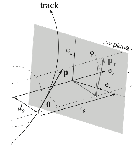
\includegraphics[width=.5\linewidth]{track_parameters}
    \caption{Perigee parameters}
    \label{fig:track_par}
\end{figure}
%%% Local Variables:
%%% mode: latex
%%% TeX-master: "../search_for_DM_LED_with_ATLAS"
%%% End:
